% Created by tikzDevice version 0.6.2-92-0ad2792 on 2013-02-14 19:21:54
% !TEX encoding = UTF-8 Unicode
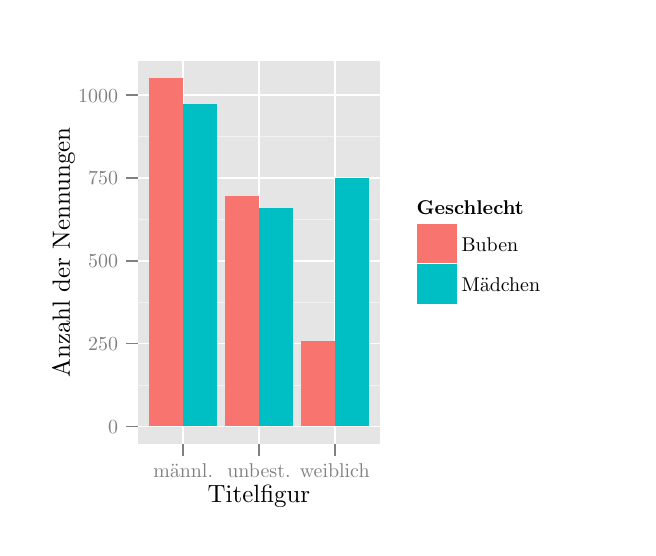
\begin{tikzpicture}[x=1pt,y=1pt]
\definecolor[named]{fillColor}{rgb}{1.00,1.00,1.00}
\path[use as bounding box,fill=fillColor,fill opacity=0.00] (0,0) rectangle (216.81,180.67);
\begin{scope}
\path[clip] (  0.00,  0.00) rectangle (216.81,180.67);
\definecolor[named]{drawColor}{rgb}{1.00,1.00,1.00}
\definecolor[named]{fillColor}{rgb}{1.00,1.00,1.00}

\path[draw=drawColor,line width= 0.6pt,line join=round,line cap=round,fill=fillColor] (  0.00,  0.00) rectangle (216.81,180.67);
\end{scope}
\begin{scope}
\path[clip] ( 39.75, 30.32) rectangle (127.38,168.63);
\definecolor[named]{fillColor}{rgb}{0.90,0.90,0.90}

\path[fill=fillColor] ( 39.75, 30.32) rectangle (127.38,168.63);
\definecolor[named]{drawColor}{rgb}{0.95,0.95,0.95}

\path[draw=drawColor,line width= 0.3pt,line join=round] ( 39.75, 51.56) --
	(127.38, 51.56);

\path[draw=drawColor,line width= 0.3pt,line join=round] ( 39.75, 81.47) --
	(127.38, 81.47);

\path[draw=drawColor,line width= 0.3pt,line join=round] ( 39.75,111.38) --
	(127.38,111.38);

\path[draw=drawColor,line width= 0.3pt,line join=round] ( 39.75,141.29) --
	(127.38,141.29);
\definecolor[named]{drawColor}{rgb}{1.00,1.00,1.00}

\path[draw=drawColor,line width= 0.6pt,line join=round] ( 39.75, 36.60) --
	(127.38, 36.60);

\path[draw=drawColor,line width= 0.6pt,line join=round] ( 39.75, 66.51) --
	(127.38, 66.51);

\path[draw=drawColor,line width= 0.6pt,line join=round] ( 39.75, 96.42) --
	(127.38, 96.42);

\path[draw=drawColor,line width= 0.6pt,line join=round] ( 39.75,126.33) --
	(127.38,126.33);

\path[draw=drawColor,line width= 0.6pt,line join=round] ( 39.75,156.24) --
	(127.38,156.24);

\path[draw=drawColor,line width= 0.6pt,line join=round] ( 56.18, 30.32) --
	( 56.18,168.63);

\path[draw=drawColor,line width= 0.6pt,line join=round] ( 83.57, 30.32) --
	( 83.57,168.63);

\path[draw=drawColor,line width= 0.6pt,line join=round] (110.95, 30.32) --
	(110.95,168.63);
\definecolor[named]{fillColor}{rgb}{0.97,0.46,0.43}

\path[fill=fillColor] ( 43.86, 36.60) rectangle ( 56.18,162.34);
\definecolor[named]{fillColor}{rgb}{0.00,0.75,0.77}

\path[fill=fillColor] ( 56.18, 36.60) rectangle ( 68.51,153.01);
\definecolor[named]{fillColor}{rgb}{0.97,0.46,0.43}

\path[fill=fillColor] ( 71.24, 36.60) rectangle ( 83.57,119.99);
\definecolor[named]{fillColor}{rgb}{0.00,0.75,0.77}

\path[fill=fillColor] ( 83.57, 36.60) rectangle ( 95.89,115.56);
\definecolor[named]{fillColor}{rgb}{0.97,0.46,0.43}

\path[fill=fillColor] ( 98.63, 36.60) rectangle (110.95, 67.35);
\definecolor[named]{fillColor}{rgb}{0.00,0.75,0.77}

\path[fill=fillColor] (110.95, 36.60) rectangle (123.27,126.45);
\end{scope}
\begin{scope}
\path[clip] (  0.00,  0.00) rectangle (216.81,180.67);
\definecolor[named]{drawColor}{rgb}{0.50,0.50,0.50}

\node[text=drawColor,anchor=base east,inner sep=0pt, outer sep=0pt, scale=  0.72] at ( 32.64, 34.12) {0};

\node[text=drawColor,anchor=base east,inner sep=0pt, outer sep=0pt, scale=  0.72] at ( 32.64, 64.03) {250};

\node[text=drawColor,anchor=base east,inner sep=0pt, outer sep=0pt, scale=  0.72] at ( 32.64, 93.94) {500};

\node[text=drawColor,anchor=base east,inner sep=0pt, outer sep=0pt, scale=  0.72] at ( 32.64,123.85) {750};

\node[text=drawColor,anchor=base east,inner sep=0pt, outer sep=0pt, scale=  0.72] at ( 32.64,153.76) {1000};
\end{scope}
\begin{scope}
\path[clip] (  0.00,  0.00) rectangle (216.81,180.67);
\definecolor[named]{drawColor}{rgb}{0.50,0.50,0.50}

\path[draw=drawColor,line width= 0.6pt,line join=round] ( 35.49, 36.60) --
	( 39.75, 36.60);

\path[draw=drawColor,line width= 0.6pt,line join=round] ( 35.49, 66.51) --
	( 39.75, 66.51);

\path[draw=drawColor,line width= 0.6pt,line join=round] ( 35.49, 96.42) --
	( 39.75, 96.42);

\path[draw=drawColor,line width= 0.6pt,line join=round] ( 35.49,126.33) --
	( 39.75,126.33);

\path[draw=drawColor,line width= 0.6pt,line join=round] ( 35.49,156.24) --
	( 39.75,156.24);
\end{scope}
\begin{scope}
\path[clip] (  0.00,  0.00) rectangle (216.81,180.67);
\definecolor[named]{drawColor}{rgb}{0.50,0.50,0.50}

\path[draw=drawColor,line width= 0.6pt,line join=round] ( 56.18, 26.05) --
	( 56.18, 30.32);

\path[draw=drawColor,line width= 0.6pt,line join=round] ( 83.57, 26.05) --
	( 83.57, 30.32);

\path[draw=drawColor,line width= 0.6pt,line join=round] (110.95, 26.05) --
	(110.95, 30.32);
\end{scope}
\begin{scope}
\path[clip] (  0.00,  0.00) rectangle (216.81,180.67);
\definecolor[named]{drawColor}{rgb}{0.50,0.50,0.50}

\node[text=drawColor,anchor=base,inner sep=0pt, outer sep=0pt, scale=  0.72] at ( 56.18, 18.24) {männl.};

\node[text=drawColor,anchor=base,inner sep=0pt, outer sep=0pt, scale=  0.72] at ( 83.57, 18.24) {unbest.};

\node[text=drawColor,anchor=base,inner sep=0pt, outer sep=0pt, scale=  0.72] at (110.95, 18.24) {weiblich};
\end{scope}
\begin{scope}
\path[clip] (  0.00,  0.00) rectangle (216.81,180.67);
\definecolor[named]{drawColor}{rgb}{0.00,0.00,0.00}

\node[text=drawColor,anchor=base,inner sep=0pt, outer sep=0pt, scale=  0.90] at ( 83.57,  9.03) {Titelfigur};
\end{scope}
\begin{scope}
\path[clip] (  0.00,  0.00) rectangle (216.81,180.67);
\definecolor[named]{drawColor}{rgb}{0.00,0.00,0.00}

\node[text=drawColor,rotate= 90.00,anchor=base,inner sep=0pt, outer sep=0pt, scale=  0.90] at ( 15.23, 99.47) {Anzahl der Nennungen};
\end{scope}
\begin{scope}
\path[clip] (  0.00,  0.00) rectangle (216.81,180.67);
\definecolor[named]{fillColor}{rgb}{1.00,1.00,1.00}

\path[fill=fillColor] (136.25, 76.46) rectangle (195.90,122.49);
\end{scope}
\begin{scope}
\path[clip] (  0.00,  0.00) rectangle (216.81,180.67);
\definecolor[named]{drawColor}{rgb}{0.00,0.00,0.00}

\node[text=drawColor,anchor=base west,inner sep=0pt, outer sep=0pt, scale=  0.72] at (140.52,113.25) {\bfseries Geschlecht};
\end{scope}
\begin{scope}
\path[clip] (  0.00,  0.00) rectangle (216.81,180.67);
\definecolor[named]{drawColor}{rgb}{1.00,1.00,1.00}
\definecolor[named]{fillColor}{rgb}{0.95,0.95,0.95}

\path[draw=drawColor,line width= 0.6pt,line join=round,line cap=round,fill=fillColor] (140.52, 95.18) rectangle (154.97,109.64);
\end{scope}
\begin{scope}
\path[clip] (  0.00,  0.00) rectangle (216.81,180.67);
\definecolor[named]{fillColor}{rgb}{0.97,0.46,0.43}

\path[fill=fillColor] (140.52, 95.18) rectangle (154.97,109.64);

\path[] (140.52, 95.18) --
	(154.97,109.64);
\end{scope}
\begin{scope}
\path[clip] (  0.00,  0.00) rectangle (216.81,180.67);
\definecolor[named]{drawColor}{rgb}{1.00,1.00,1.00}
\definecolor[named]{fillColor}{rgb}{0.95,0.95,0.95}

\path[draw=drawColor,line width= 0.6pt,line join=round,line cap=round,fill=fillColor] (140.52, 80.73) rectangle (154.97, 95.18);
\end{scope}
\begin{scope}
\path[clip] (  0.00,  0.00) rectangle (216.81,180.67);
\definecolor[named]{fillColor}{rgb}{0.00,0.75,0.77}

\path[fill=fillColor] (140.52, 80.73) rectangle (154.97, 95.18);

\path[] (140.52, 80.73) --
	(154.97, 95.18);
\end{scope}
\begin{scope}
\path[clip] (  0.00,  0.00) rectangle (216.81,180.67);
\definecolor[named]{drawColor}{rgb}{0.00,0.00,0.00}

\node[text=drawColor,anchor=base west,inner sep=0pt, outer sep=0pt, scale=  0.72] at (156.78, 99.93) {Buben};
\end{scope}
\begin{scope}
\path[clip] (  0.00,  0.00) rectangle (216.81,180.67);
\definecolor[named]{drawColor}{rgb}{0.00,0.00,0.00}

\node[text=drawColor,anchor=base west,inner sep=0pt, outer sep=0pt, scale=  0.72] at (156.78, 85.48) {Mädchen};
\end{scope}
\end{tikzpicture}
